La función de entrada en una neurona artificial es el cálculo ponderado de las señales de entrada que recibe la neurona antes de aplicar una función de activación para producir la salida. En términos simples, la función de entrada representa cómo se combinan y procesan las entradas para determinar la actividad de la neurona.

En una neurona artificial básica, la función de entrada realiza alguna operación matemática conveniente, generalmente la suma de las señales de entrada multiplicadas por sus respectivos pesos. Esta suma ponderada se representa en la ecuación \ref{eq:e1}:

\begin{equation} \label{eq:e1} 
	Entrada = w_1x_1 + w_2x_2 + \cdots + w_nx_n + b 
\end{equation}

Donde : 
\begin{itemize}
\item $w_1, w_2, \ldots, w_n$ son los pesos asociados a cada señal de entrada $x_1, x_2, \ldots, x_n$ respectivamente.
\item $b$ es el sesgo (bias), un parametro adicional que se suma a la suma ponderada
\end{itemize}

\begin{figure}[h!]
	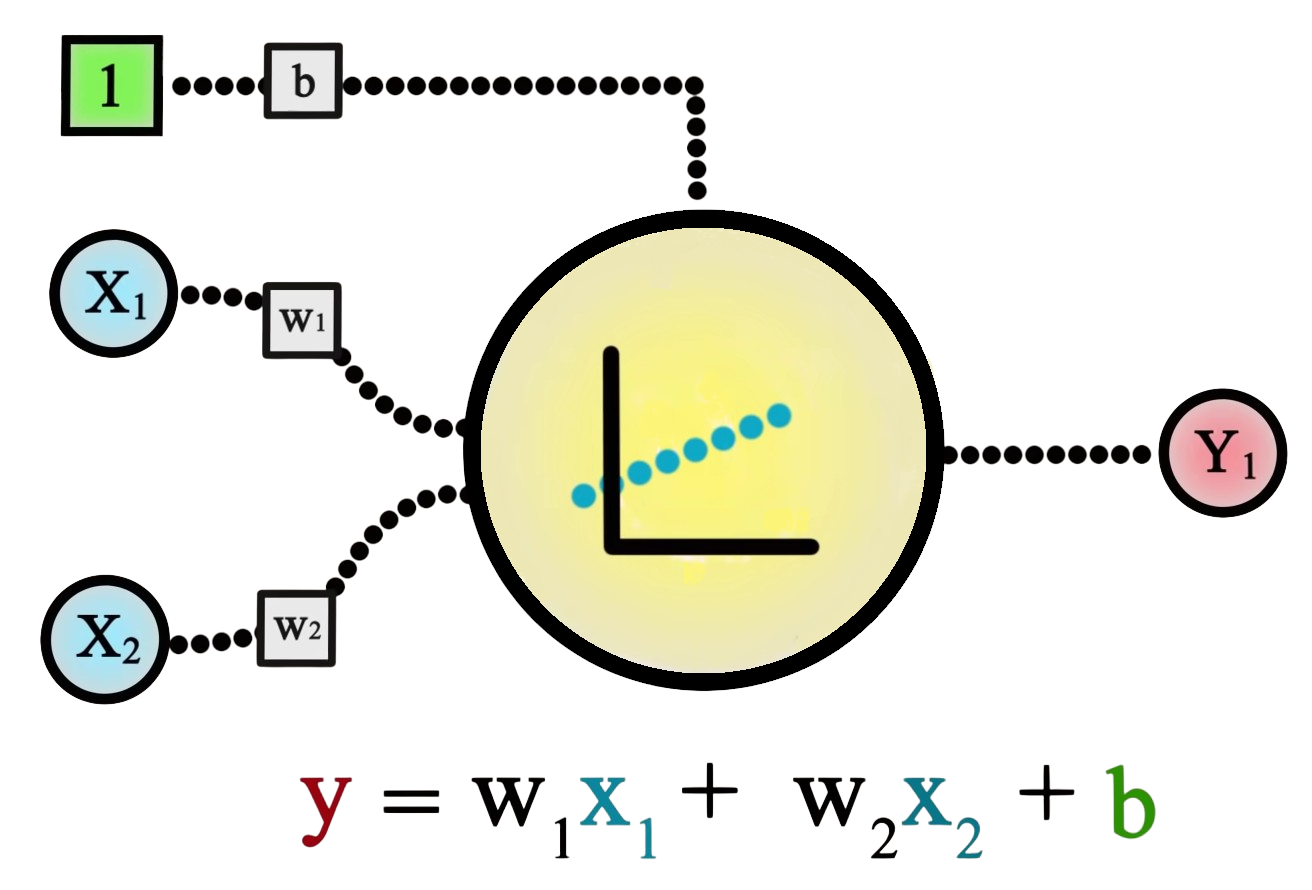
\includegraphics[width=0.65\textwidth]{capitulo2/figuras/an6.png}
	\caption[Representacion de una neurona artificial]{Representacion de una neurona artificial
		\\\textit{Fuente: Elaboracion Propia}}
	\label{fig:an6}
\end{figure}

Los pesos indican la importancia relativa de cada entrada en la determinación de la salida de la neurona, es decir, que permiten que un gran valor de entrada tenga solamente una pequeña influencia, si estos son lo suficientemente pequeños. El sesgo o bias es un término independiente que permite desplazar la función de entrada, lo que puede ser crucial para el aprendizaje y la adaptación de la red neuronal. Ver Figura \ref{fig:an6}. La función de entrada, en esencia, realiza un procesamiento lineal de las entradas ponderadas por sus pesos. Posteriormente, esta suma ponderada se introduce en una función de activación.

